\subsection{Robôs escaladores}\label{sota_climbers}
%TODO ROBICEN
Robôs escaladores são sistemas capazes de sustentar seu próprio peso contra a
gravidade, movendo-se em simples ou complexas estruturas geométricas, como
paredes, tetos e telhados, palhetas de turbinas e plantas nucleares.
Essa classe de robôs oferece eficiência operacional em ambientes
de alta periculosidade, sendo utilizados visando saúde e segurança dos
trabalhadores, como em inspeção e limpeza de arranha-céus, diagnóstico de
tanques de armazenamento em plantas nucleares, solda e manutenção de cascos de
navios e palhetas de turbinas \cite{clawar}.

Os grandes desafios nos projetos de sistemas escaladores são mobilidade e
aderência, além de consumo de energia, capacidade de carga e peso. Em
\cite{modular}e \cite{climbsurv}, os robôs escaladores são divididos em tipos de locomoção:
pernas, como andador, utilizando segmentos deslizantes, rodas, esteiras, avanço
pendurado por braços, por cabos e biomimética; e categorias de adesão: sucção ou
pneumática, magnética, eletrostática, química, preensão e híbrida.

No caso específico deste estudo da arte, destacam-se os robôs escaladores com as
seguintes aplicações:

\begin{itemize}
  \item \emph{Construção de navios e turbinas}: RRX3 para soldagem
  \citep{rrx3}, \emph{Climbing Robot for Grit Blasting} para limpeza
  \citep{crgb} e ICM Robot para inspeção \citep{icm};
  \item \emph{Construção industrial}: ROMA II \citep{roma} e
  CROMSCI \citep{CROMSCI}, ambos para inspeção; 
 \item \emph{Planta petroquímica}: ROBICEN \citep{robicen} e
  TRIPILLAR \citep{tripillar}, ambos para inspeção.  
\end{itemize}

O RRX3 (figura~\ref{rrx3}), Daewoo Shipbuilding and Marine Engineering, é um
robô para a soldagem de casco de navios. Possui adesão por preensão, locomoção transversal utilizando segmentos deslizantes e locomoção
longitudinal por rodas. Possui um manipulador de 1.5 m com três juntas
prismáticas e três juntas de revolução (3P3R) para a operação de soldagem. Suas
principais vantagens e desvantagens em relação à aplicação HVOF são:

\begin{figure}[ht]
\centering
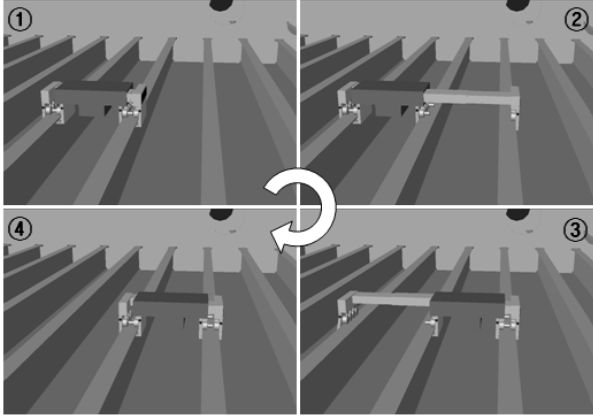
\includegraphics[width=8.4cm]{figs/climbers/RRX3_moving.jpg}
\caption{Translação horizontal do robô RRX3.}
\label{rrx3}
\end{figure}

\textbf{Vantagens:}
\begin{itemize}
  \item Base com capacidade de carga 120 kg;
  \item Manipulador com capacidade de carga 5 kg;
  \item Manipulador de precisão milimétrica;
  \item Robô robusto que trabalha com instrumento de alta temperatura (solda);
\end{itemize}

\textbf{Desvantagens:}
\begin{itemize}
  \item Locomoção restrita impede utilização em estruturas geométricas
  complexas;
  \item Manipulador não possui alcance suficiente para a aplicação fim;
  \item Manipulador com efetuador de baixa velocidade;
\end{itemize}

O \emph{Climbing robot for Grit Blasting} (figura~\ref{grit}), University of
Coruna, é um robô para jateamento abrasivo em navios. O robô utiliza duas plataformas deslizantes com sistema de adesão por
ímã magnético. Os módulos apresentam movimentação relativa entre si e pode rotar
para compensar as curvaturas do casco do navio ou desviar de objetos. 

\begin{figure}[ht]
\centering
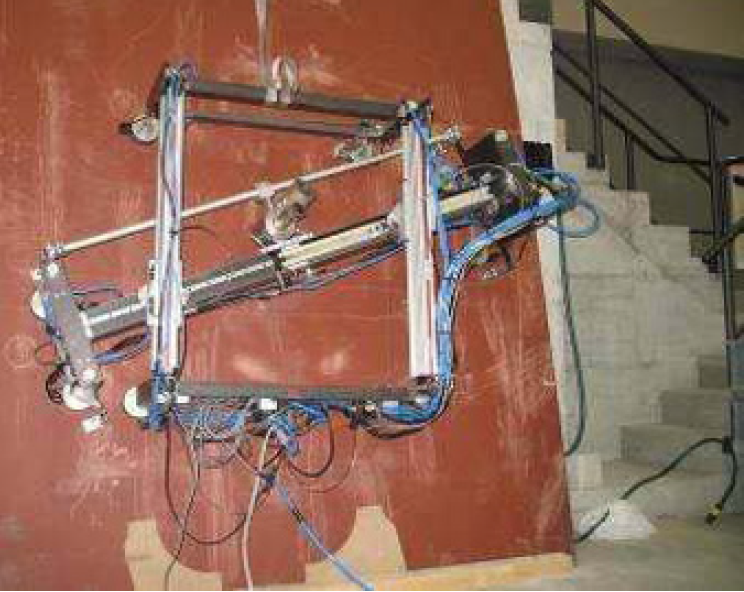
\includegraphics[width=8.4cm]{figs/climbers/grit.png}
\caption{Climbing robot for Grit Blasting}
\label{grit}
\end{figure}

\textbf{Vantagens:}
\begin{itemize}
  \item Base com capacidade de carga de sistema abrasivo semelhante ao HVOF;
  \item Base com locomoção de precisão milimétrica;
\end{itemize}

\textbf{Desvantagens:}
\begin{itemize}
  \item Locomoção ampla, porém não aplicável às estruturas geométricas
  complexas. A curvatura do casco é simples quando comparada à pá da turbina;
  \item Não possui manipulador, logo o sistema deve percorrer todo o
  casco;
  \item A instalação de um manipulador prejudica a estabilidade do sistema;
\end{itemize}

\emph{The Climber} (figura~\ref{icm}), ICM Robotics, é um robô para inspeção de
turbinas eólicas, remoção de revestimento, limpeza de superfície, e aplicação de revestimento.
Possui adesão pneumática (sucção) e locomoção por esteiras. 

\begin{figure}[ht]
\centering
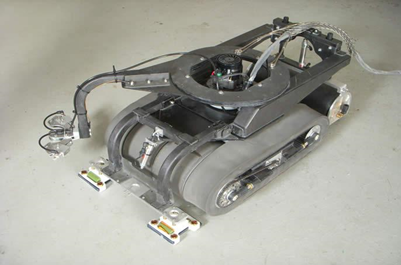
\includegraphics[width=8.4cm]{figs/climbers/icm.png}
\caption{Robô The Climber da ICM Robotics}
\label{icm}
\end{figure}

\textbf{Vantagens:}
\begin{itemize}
  \item Base com capacidade de carga de 25 kg;
  \item Base com locomoção de precisão milimétrica;
  \item Manipulador para revestimento HVOF pode ser acoplado à base; 
\end{itemize}

\textbf{Desvantagens:}
\begin{itemize}
  \item Manipulador com baixo alcance;
  \item Manipulador com efetuador de baixa velocidade;;
  \item Locomoção apresenta restrição a certas curvaturas devido às esteiras;
\end{itemize}

O ROMA II (figura~\ref{roma2}), Universidade Carlos II de Madrid, é um robô para
inspeção de ambientes complexos. A sua tecnologia de adesão é pneumática (sucção) e
locomove-se como uma lagarta (biomimética). Sua movimentação e planejamento de
trajetória são realizados de maneira ótima de forma a garantir estabilidade e
evitar obstáculos. 

\begin{figure}[ht]
\centering
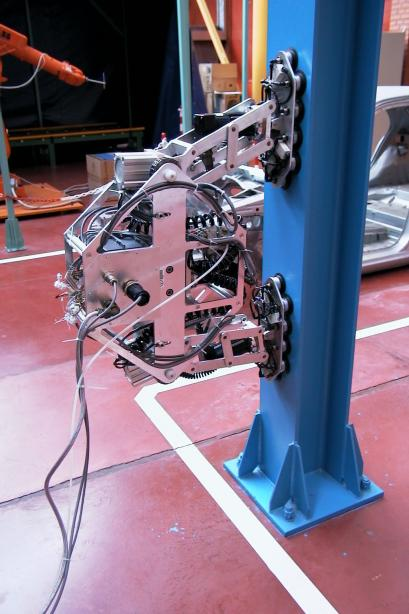
\includegraphics[width=8.4cm]{figs/climbers/roma2.jpg}
\caption{ROMA II.}
\label{roma2}
\end{figure}

\textbf{Vantagens:}
\begin{itemize}
  \item Base com grande capacidade de carga;
  \item Base com locomoção de grande precisão;
  \item Movimenta-se em ambientes de grande complexidade geométrica; 
\end{itemize}

\textbf{Desvantagens:}
\begin{itemize}
  \item Não possui manipulador para aplicação HVOF;
  \item A instalação de um manipulador irá desequilibrar o sistema,
  principalmente durante a locomoção;
\end{itemize}


CROMSCI (figura~\ref{cromsci}), Kaiserslautern University of Technology, é um
robô autônomo para inspeção de grandes paredes de concreto, como pilares de pontes, barragens. Seu
sistema de adesão é composto por sete câmaras de vácuo (sucção), com um sistema
de controle por válvulas e sensores de pressão para reagir rapidamaente a
condições adversas. Locomove-se com rodas omnidirecionais para locomoção.

\begin{figure}[ht]
\centering
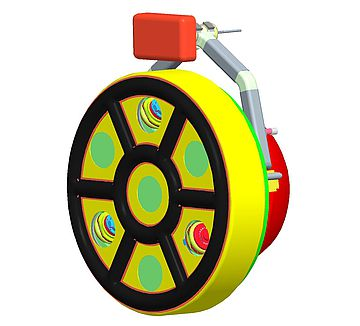
\includegraphics[width=8.4cm]{figs/climbers/cromsci.jpg}
\caption{Robô CROMSCI.}
\label{cromsci}
\end{figure}

\textbf{Vantagens:}
\begin{itemize}
  \item Base com locomoção de precisão milimétrica; 
\end{itemize}

\textbf{Desvantagens:}
\begin{itemize}
  \item Manipulador com alcance de 80 cm;
  \item Manipulador com efetuador de baixa velocidade;
  \item Protótipo ainda com pouca capacidade de carga;
\end{itemize}

Planta petroquímica: ROBICEN

TRIPILLAR (figura~\ref{tripillar}), École polytechnique fédérale de Lausanne, é
um robô escalador de pequeno porte (96 x 46 x 64 mm) desenvolvido para a inspeção de plantas
petroquímicas. Utiliza um sistema como pernas de lagarta magnéticas em um
formato triangular. Locomove-sepor esteiras.

\begin{figure}[ht]
\centering
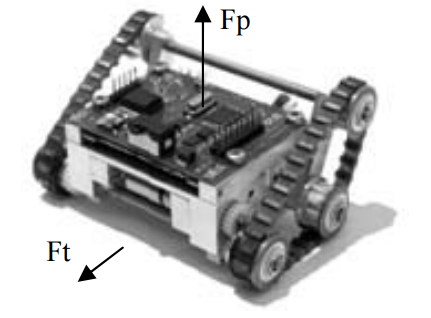
\includegraphics[width=8.4cm]{figs/climbers/tripillar.png}
\caption{Robô TRIPILLAR.}
\label{tripillar}
\end{figure}

\textbf{Vantagens:}
\begin{itemize}
  \item Base com locomoção de precisão milimétrica;
  \item Sistema robusto;
  \item Controle simples;
  \item Pequenas dimensões; 
\end{itemize}

\textbf{Desvantagens:}
\begin{itemize}
  \item Não foi testado em estruturas de grande complexidade geométrica; 
  \item Não apresenta manipulador;
  \item Protótipo ainda com pouca capacidade de carga;
\end{itemize}
   
Os robôs escaladores são utilizados em diversas aplicações e possuem diferentes
soluções de aderência e locomoção, como foi exposto nesta subseção. Não há,
até o momento, um robô escalador que possui todas as características
exigidas para a tarefa de HVOF em pás de turbinas, porém a adaptação de
alguns desses sistemas, como \emph{The Climber} da ICM Robotic, pode gerar
soluções completas.
